\chapter{Experimentos y Resultados}
\label{experimentacion}
\section{Introducci'on}

A los efectos de probar el desempe'no del Proxy, se dise'no un experimento con sitios reales para simular un ambiente adecuado para la prueba. Se extrajeron sitios del Top de Alexa\footnote{http://www.alexa.com/}, que es una compan'ia de Amazon\footnote{http://www.amazon.com} que se especializa en realizar mediciones de tr'afico global y brinda las estad'isticas obtenidas. Tambi'en, ofrece un Ranking Global de los sitios m'as visitados de toda Internet, de este Ranking se extrajeron los sitios para la experimentaci'on. Se desarrollaron herramientas para extraer una porci'on del Ranking de Alexa y tambi'en para automatizar el experimento en s'i.

\section{Ranking de Alexa}
\label{rankingalexa}
El Ranking de Alexa se encuentra online en su sitio, pero fue necesario desarrollar una peque'na aplicaci'on para extraer el listado y guardarlo en un archivo de texto para su posterior uso. Esta herramienta se encuentra disponible en Github \citep{alexatop}.

\section{Chrome-har-capturer}

Con la idea de automatizar el experimento, se utiliz'o \emph{Chrome-har-capturer} \citep{harcapturer} que, a trav'es de la API de depuraci'on remota (ver \citep{debugger}) del Navegador Chrome o Chromium, permite que la herramienta pueda interactuar con dicha aplicaci'on. Esto permite  poder navegar un sitio en particular y obtener un archivo HAR, que contiene los resultados de la interacci'on del navegador con el sitio.

El HAR\footnote{HTTP Archive} obtenido, es un archivo con formato JSON que contiene informaci'on de la interacci'on de un navegador con un sitio \citep{harSpec}. Contiene un registro de cada objeto que est'a siendo cargado por el navegador. La informaci'on acerca de los tiempos que se puede obtener es:
\begin{enumerate}
\item Cuanto tarda en recuperar la informaci'on de DNS.
\item Cuanto tarda en peticionar un objeto.
\item Cuanto tarda en conectarse al servidor.
\item Cuanto tarda la transferencia desde el servidor al navegador de cada objeto.
\end{enumerate}

De este archivo, se pueden extraer 2 valores que son importantes para evaluar el tiempo de carga de los sitios. Estos valores son:
\begin{enumerate}
\item onContentLoad: Tiempo en el que el contenido del sitio se carga.
\item onLoad: Tiempo en el que es sitio se carga seg'un el navegador.
\end{enumerate}

De los cuales, tomaremos como referencia \emph{onLoad} ya que es el tiempo m'as cercano a la experiencia que tiene un usuario final cuando navega el sitio en cuesti'on. Es decir, es el valor que est'a m'as cerca de lo que tarda el Navegador en renderizar el sitio completo.

\section{Experimento}

El experimento consiste en un Navegador conectado a Internet a trav'es del Proxy, en el cual se realiza la petici'on de la p'agina de inicio, con todos sus elementos, de ciertos sitios seleccionados. Se divide en 2 fases, en una, las peticiones se realizan en HTTP plano, y en otra en HTTPS, es decir, que el cliente se conecta de forma segura al Proxy. Con el fin de poder realizar la comparaci'on con un Proxy Transparente (ver Cap'itulo \ref{proxy}), fu'e necesario realizar ciertas modificaciones en la versi'on del Proxy desarrollado, para quitarle toda la inteligencia de selecci'on de m'etodos, y as'i poder tener un Proxy alternativo para realizar la experiencia. Cada una de las fases se realiz'o con el Proxy desarrollado y con el Proxy Transparente.

La primera fase puede verse en las Figuras \ref{httpNormal} y \ref{httpOptimizado}.

\begin{figure}[h]
  	\centering
	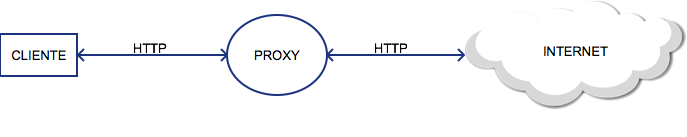
\includegraphics[width=\textwidth]{img/httpNormal}
	\caption{\small HTTP - Proxy Transparente}
	\label{httpNormal}
\end{figure}

\begin{figure}[h]
  	\centering
	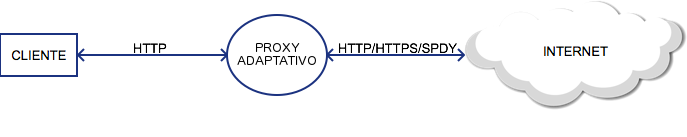
\includegraphics[width=\textwidth]{img/httpOptimizado}
	\caption{\small HTTP - Proxy Adaptativo}
	\label{httpOptimizado}
\end{figure}

En la segunda fase en las im'agenes \ref{httpsNormal} y \ref{httpsOptimizado}.

\begin{figure}[h]
  	\centering
	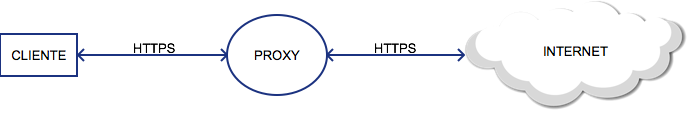
\includegraphics[width=\textwidth]{img/httpsNormal}
	\caption{\small HTTPS - Proxy Transparente}
	\label{httpsNormal}
\end{figure}

\begin{figure}[h]
  	\centering
	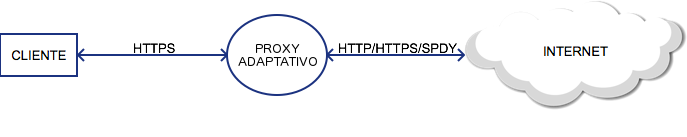
\includegraphics[width=\textwidth]{img/httpsOptimizado}
	\caption{\small HTTPS - Proxy Adaptativo}
	\label{httpsOptimizado}
\end{figure}

Se seleccionaron 200 sitios extra'idos del Ranking de Alexa, utilizando la herramienta vista en la Secci'on \ref{rankingalexa}. El listado completo para HTTP y HTTPS se puede ver en la Secci'on \ref{sitiosAlexa} de los Ap'endices.

Previo a iniciar el experimento, se obtuvieron todos los Protocolos Soportados de los sitios seleccionados, as'i tambi'en como el RTT de los mismos. De esta manera, el Proxy ya tiene a priori, algo de informaci'on para poder determinar que Protocolo va a utilizar para obtener el sitio.

Se dise'n'o un script para automatizar el experimento. Este lee de un archivo de texto el listado de los sitios del correspondiente protocolo, realiza la petici'on a trav'es de Chrome, y guarda el archivo HAR generado en una carpeta.

\begin{pseudocode}{Experimento}{ }
\BEGIN
	\FOR sitio \in sitios \DO \\
	\BEGIN
		iniciar\ chrome\ a\ traves\ del\ proxy\\
		ejecutar\ chrome-har-capturer\\
		cerrar\ chrome\\
	\END
\END
\end{pseudocode}

Una vez obtenidos todos los archivos de las pruebas, se procesaron para extraer los valores de onConcentLoad y onLoad. Los resultados se encuentran disponibles en el repositorio del presente trabajo \citep{tfl}.

\section{Resultados}

En los resultados se observa que, a lo largo de todos los sitios, el rendimiento del Proxy Adaptativo es mejor o similar en algunos casos que el Proxy Transparente. De los sitios seleccionados para la fase de HTTP, 60 soportan los 3 protocolos, de los cuales en 45 sitios el Proxy opt'o por utilizar SPDY. De los sitios de la fase de HTTPS, 75 soportan los 3 protocolos, y en 53 fu'e seleccionado SPDY.

En el caso de HTTP, puede observarse una mejora promedio de un 5\%, con picos de hasta un 17\%. La vista general de los sitios que soportan los 3 protocolos puede verse en la Figura \ref{resGralHTTP}.

\begin{figure}[h!]
  	\centering
	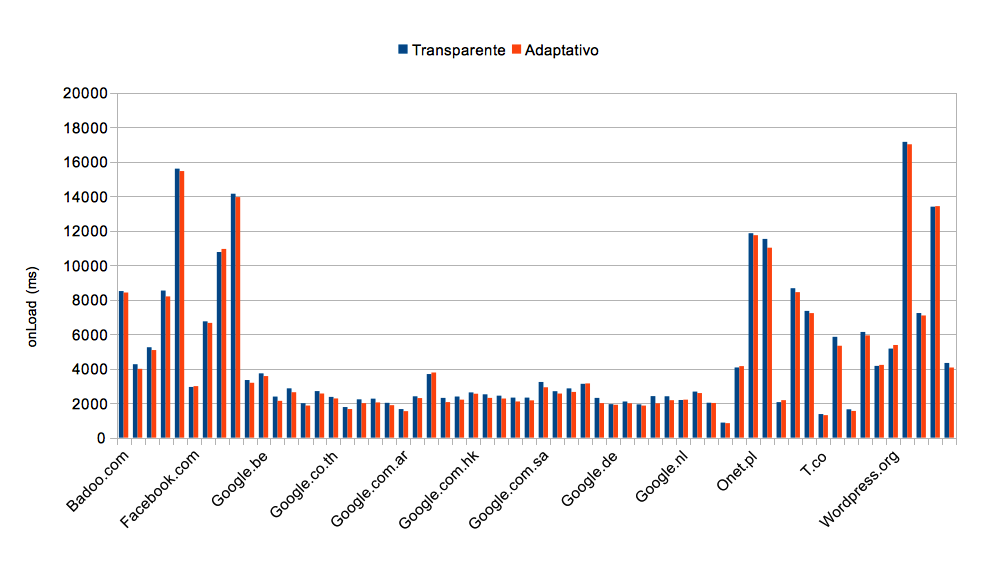
\includegraphics[width=\textwidth]{img/resGralHTTP}
	\caption{\small Resultados HTTP - Sitios con todos los protocolos soportados}
	\label{resGralHTTP}
\end{figure}

En los sitios que se seleccion'o como protocolo a SPDY, la mejora promedio fue del 6\%.
 
 \begin{figure}[h!]
  	\centering
	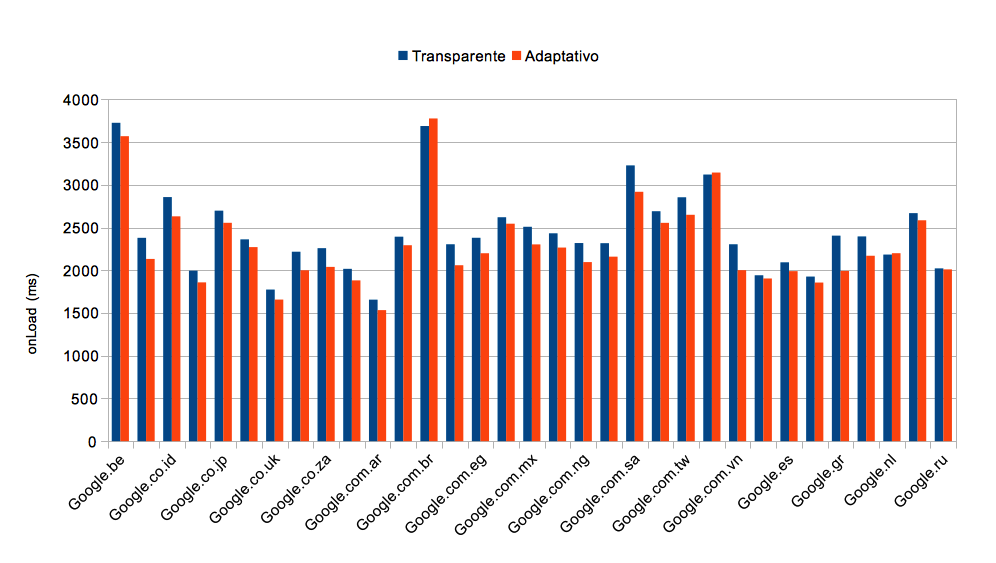
\includegraphics[width=\textwidth]{img/resGoogleHTTP}
	\caption{\small Resultados HTTP - Sitios del dominio Google}
	\label{resGoogleHTTP}
\end{figure}

En el caso de HTTPS, puede observarse una mejora promedio de un 7\%, con picos de hasta un 24\%.

\begin{figure}[h!]
  	\centering
	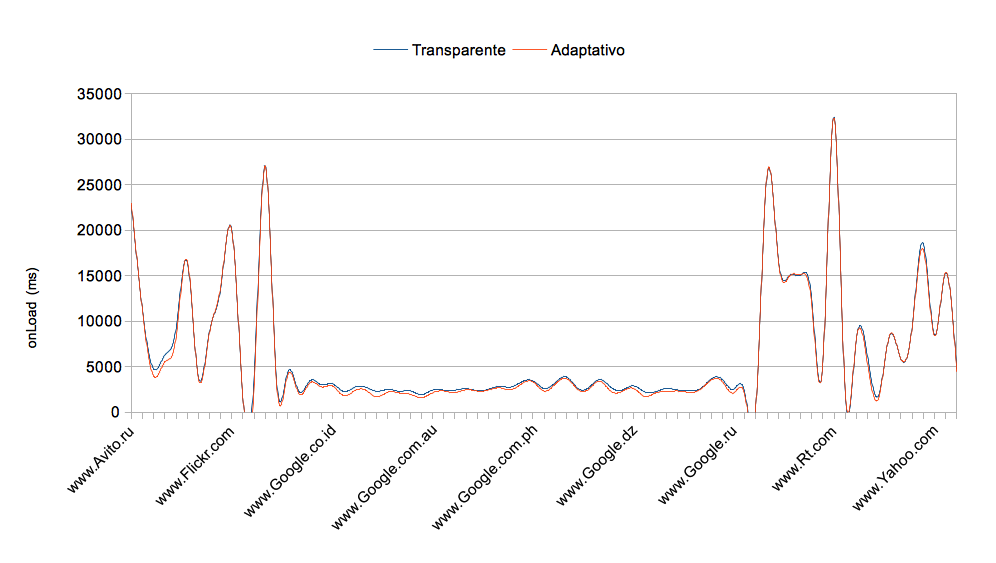
\includegraphics[width=\textwidth]{img/resGralHTTPS}
	\caption{\small Resultados HTTPS - Sitios con todos los protocolos soportados}
	\label{resGralHTTPS}
\end{figure}

En los sitios que se seleccion'o como protocolo a SPDY, la mejora promedio fue del 10\%.

\begin{figure}[h!]
  	\centering
	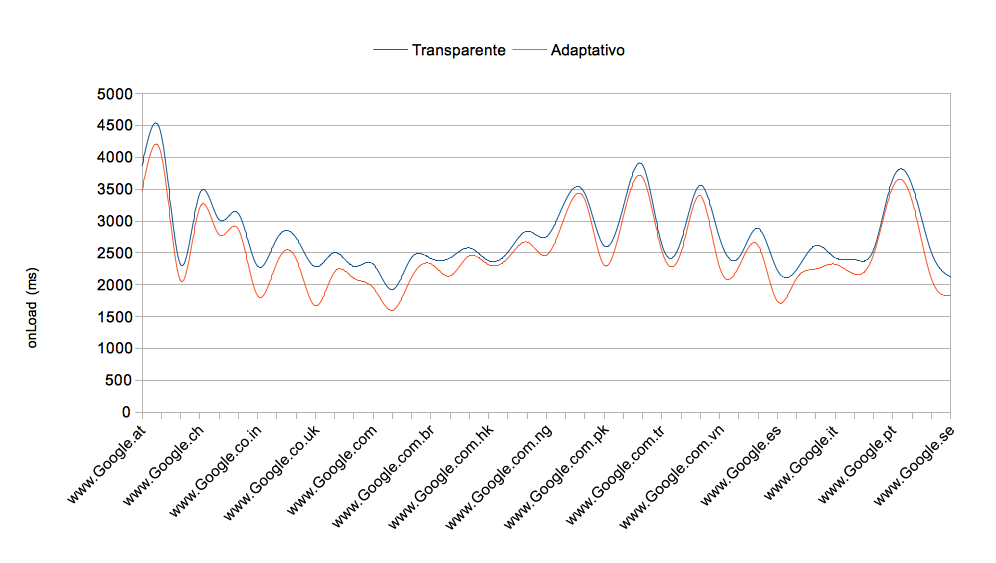
\includegraphics[width=\textwidth]{img/resGoogleHTTPS}
	\caption{\small Resultados HTTPS - Sitios del dominio Google}
	\label{resGoogleHTTPS}
\end{figure}

